% Appendix E: Veilid Developer Correspondence
\section{Veilid Developer Correspondence}
\label{app:veilid-correspondence}

This appendix reproduces excerpts from the public Veilid Discord server.
These messages from Christien Rioux (DilDog), lead developer of the Veilid
framework, informed architectural decisions in this project.

\begin{figure}[H]
\centering
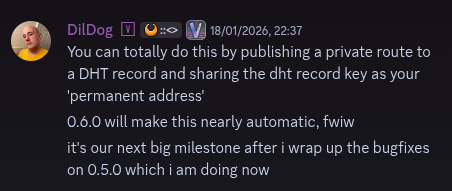
\includegraphics[width=0.7\textwidth]{Figures/screenshots/veilid1.png}
\caption{DilDog on publishing private routes via DHT records as a
  ``permanent address'' pattern, and the planned v0.6.0 automation of this
  mechanism (January 2026).}
\label{fig:veilid-discord-1}
\end{figure}

\begin{figure}[H]
\centering
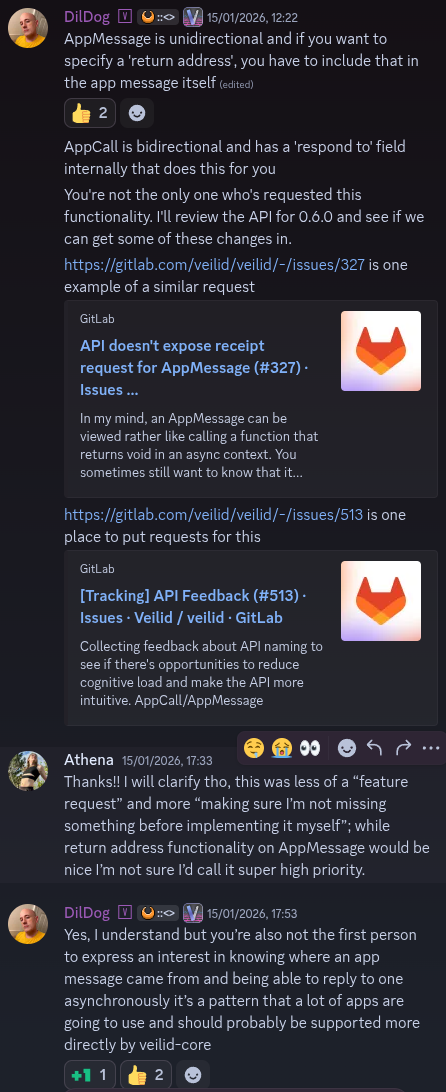
\includegraphics[width=\textwidth,height=0.8\textheight,keepaspectratio]{Figures/screenshots/veilid2.png}
\caption{Discussion of \texttt{app\_call} vs.\ \texttt{app\_message}
  semantics: \texttt{app\_call} is bidirectional with a response, while
  \texttt{app\_message} is fire-and-forget with no delivery guarantee.}
\label{fig:veilid-discord-2}
\end{figure}

\begin{figure}[H]
\centering
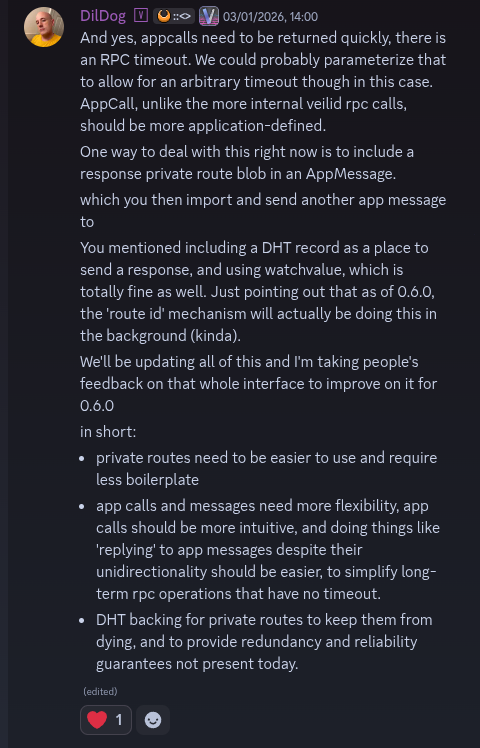
\includegraphics[width=0.7\textwidth]{Figures/screenshots/veilid3.png}
\caption{DilDog on planned improvements to the Veilid API: private route
  resilience, provider routing, and DHT publishing of route blobs.}
\label{fig:veilid-discord-3}
\end{figure}

\begin{figure}[H]
\centering
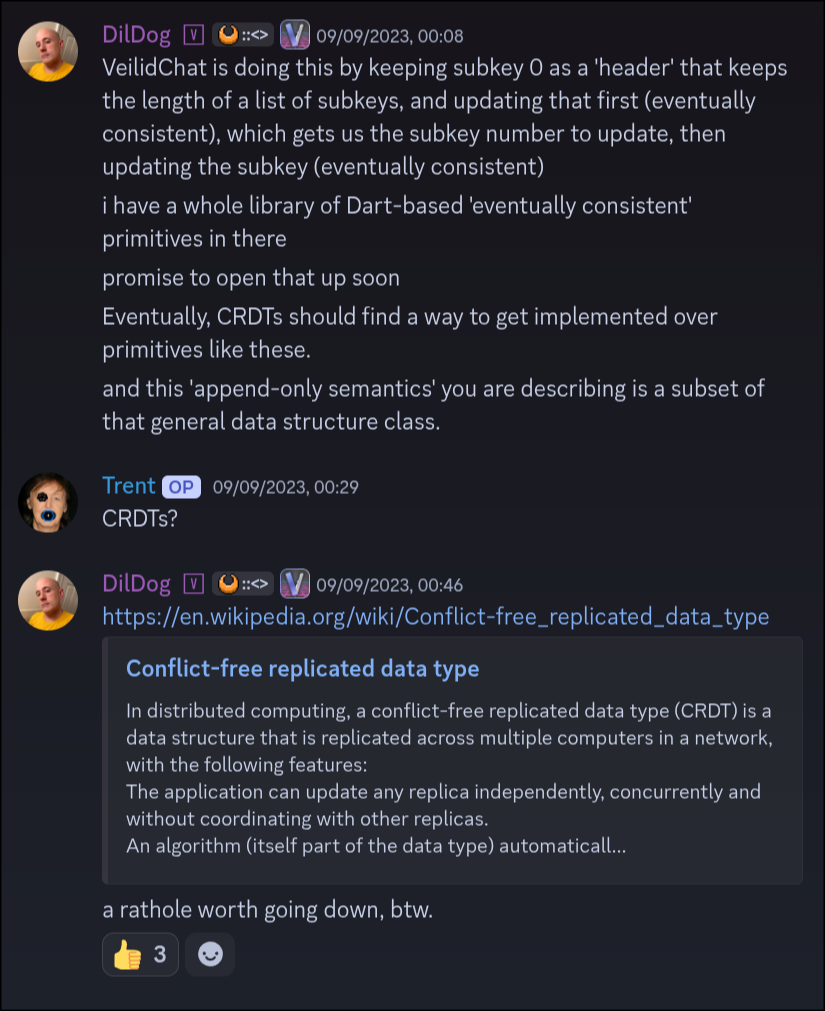
\includegraphics[width=0.7\textwidth]{Figures/screenshots/veilid4.png}
\caption{DilDog on DHT record design patterns: using subkey~0 as a header
  for eventually consistent updates, and the relationship to CRDTs.}
\label{fig:veilid-discord-4}
\end{figure}

\begin{figure}[H]
\centering
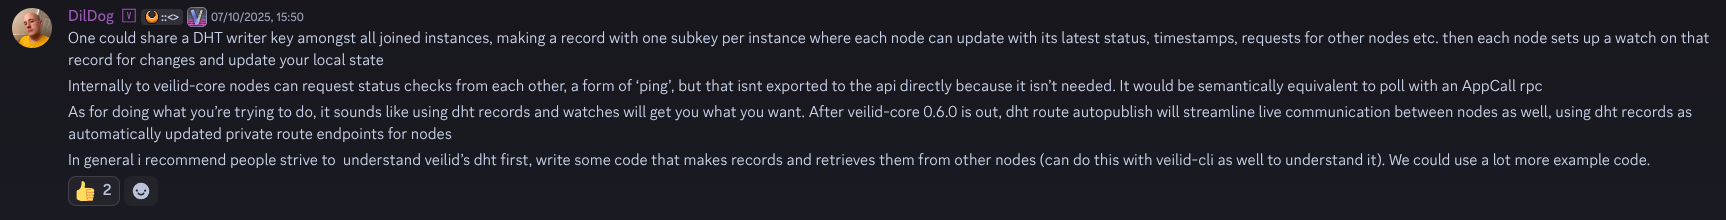
\includegraphics[width=\textwidth]{Figures/screenshots/veilid5.png}
\caption{DilDog on DHT record ownership and multi-writer patterns: each
  node can own a record and update its subkeys independently, with
  eventual consistency across the network.}
\label{fig:veilid-discord-5}
\end{figure}
